\documentclass{article}

%%%% packages and definitions (optional)
\usepackage{graphicx} % allows inclusion of graphics
\usepackage{graphics}
\usepackage{placeins}
\usepackage{booktabs} % nice rules (thick lines) for tables
\usepackage{microtype} % improves typography for PDF
\usepackage{xspace}
\usepackage[hidelinks]{hyperref}
\usepackage{xspace}
\usepackage{hhline}

\usepackage{tabularx}
\newcolumntype{b}{X}
\newcolumntype{s}{>{\hsize=.5\hsize}X}
\newcolumntype{m}{>{\hsize=.75\hsize}X}

\newcommand{\SN}{S$_N$}
\renewcommand{\vec}[1]{\bm{#1}} %vector is bold italic
\newcommand{\vd}{\bm{\cdot}} % slightly bold vector dot
\newcommand{\grad}{\vec{\nabla}} % gradient
\newcommand{\ud}{\mathop{}\!\mathrm{d}} % upright derivative symbol
\newcommand{\Cyclus}{\textsc{Cyclus}\xspace}%
\newcommand{\Cycamore}{\textsc{Cycamore}\xspace}%
\graphicspath{ {images/} }
\usepackage[affil-it]{authblk}
\usepackage{tikz}
\usetikzlibrary{positioning, arrows, decorations, shapes }
\usepackage{cleveref}

\usepackage[acronym,toc]{glossaries}
%\newacronym{<++>}{<++>}{<++>}
\newacronym[longplural={metric tons of heavy metal}]{MTHM}{MTHM}{metric ton of heavy metal}
\newacronym{ABM}{ABM}{agent-based modeling}
\newacronym{ACDIS}{ACDIS}{Program in Arms Control \& Domestic and International Security}
\newacronym{ADS}{ADS}{Accelerator-Driven Systems}
\newacronym{AHTR}{AHTR}{Advanced High Temperature Reactor}
\newacronym{ANDRA}{ANDRA}{Agence Nationale pour la gestion des D\'echets RAdioactifs, the French National Agency for Radioactive Waste Management}
\newacronym{ANL}{ANL}{Argonne National Laboratory}
\newacronym{ANS}{ANS}{American Nuclear Society}
\newacronym{API}{API}{application programming interface}
\newacronym{ARE}{ARE}{Aircraft Reactor Experiment}
\newacronym{ARFC}{ARFC}{Advanced Reactors and Fuel Cycles}
\newacronym{ASME}{ASME}{American Society of Mechanical Engineers}
\newacronym{ATWS}{ATWS}{Anticipated Transient Without Scram}
\newacronym{BDBE}{BDBE}{Beyond Design Basis Event}
\newacronym{BIDS}{BIDS}{Berkeley Institute for Data Science}
\newacronym{BWR}{BWR}{Boiling Water Reactor}
\newacronym{CAFCA}{CAFCA}{ Code for Advanced Fuel Cycles Assessment }
\newacronym{CDTN}{CDTN}{Centro de Desenvolvimento da Tecnologia Nuclear}
\newacronym{CEA}{CEA}{Commissariat \`a l'\'Energie Atomique et aux \'Energies Alternatives}
\newacronym{CI}{CI}{continuous integration}
\newacronym{CNEN}{CNEN}{Comiss\~{a}o Nacional de Energia Nuclear}
\newacronym{CNERG}{CNERG}{Computational Nuclear Engineering Research Group}
\newacronym{COSI}{COSI}{Commelini-Sicard}
\newacronym{COTS}{COTS}{commercial, off-the-shelf}
\newacronym{CSNF}{CSNF}{commercial spent nuclear fuel}
\newacronym{CTAH}{CTAHs}{Coiled Tube Air Heaters}
\newacronym{CUBIT}{CUBIT}{CUBIT Geometry and Mesh Generation Toolkit}
\newacronym{CURIE}{CURIE}{Centralized Used Fuel Resource for Information Exchange}
\newacronym{DAG}{DAG}{directed acyclic graph}
\newacronym{DANESS}{DANESS}{Dynamic Analysis of Nuclear Energy System Strategies}
\newacronym{DBE}{DBE}{Design Basis Event}
\newacronym{DESAE}{DESAE}{Dynamic Analysis of Nuclear Energy Systems Strategies}
\newacronym{DHS}{DHS}{Department of Homeland Security}
\newacronym{DOE}{DOE}{Department of Energy}
\newacronym{DRACS}{DRACS}{Direct Reactor Auxiliary Cooling System}
\newacronym{DRE}{DRE}{dynamic resource exchange}
\newacronym{DSNF}{DSNF}{DOE spent nuclear fuel}
\newacronym{DYMOND}{DYMOND}{Dynamic Model of Nuclear Development }
\newacronym{EBS}{EBS}{Engineered Barrier System}
\newacronym{EDF}{EDF}{Électricité de France}
\newacronym{EDZ}{EDZ}{Excavation Disturbed Zone}
\newacronym{EIA}{EIA}{U.S. Energy Information Administration}
\newacronym{EPA}{EPA}{Environmental Protection Agency}
\newacronym{EPR}{EPR}{European Pressurized Reactors}
\newacronym{EP}{EP}{Engineering Physics}
\newacronym{EU}{EU}{European Union}
\newacronym{FCO}{FCO}{Fuel Cycle Options}
\newacronym{FCT}{FCT}{Fuel Cycle Technology}
\newacronym{FEHM}{FEHM}{Finite Element Heat and Mass Transfer}
\newacronym{FEPs}{FEPs}{Features, Events, and Processes}
\newacronym{FHR}{FHR}{Fluoride-Salt-Cooled High-Temperature Reactor}
\newacronym{FLiBe}{FLiBe}{Fluoride-Lithium-Beryllium}
\newacronym{FP}{FP}{Fission Products}
\newacronym{GDSE}{GDSE}{Generic Disposal System Environment}
\newacronym{GDSM}{GDSM}{Generic Disposal System Model}
\newacronym{GENIUSv1}{GENIUSv1}{Global Evaluation of Nuclear Infrastructure Utilization Scenarios, Version 1}
\newacronym{GENIUSv2}{GENIUSv2}{Global Evaluation of Nuclear Infrastructure Utilization Scenarios, Version 2}
\newacronym{GENIUS}{GENIUS}{Global Evaluation of Nuclear Infrastructure Utilization Scenarios}
\newacronym{GPAM}{GPAM}{Generic Performance Assessment Model}
\newacronym{GRSAC}{GRSAC}{Graphite Reactor Severe Accident Code}
\newacronym{GUI}{GUI}{graphical user interface}
\newacronym{HLW}{HLW}{high level waste}
\newacronym{HPC}{HPC}{high-performance computing}
\newacronym{HTC}{HTC}{high-throughput computing}
\newacronym{HTGR}{HTGR}{High Temperature Gas-Cooled Reactor}
\newacronym{IAEA}{IAEA}{International Atomic Energy Agency}
\newacronym{IEMA}{IEMA}{Illinois Emergency Mangament Agency}
\newacronym{IHLRWM}{IHLRWM}{International High Level Radioactive Waste Management}
\newacronym{INL}{INL}{Idaho National Laboratory}
\newacronym{IPRR1}{IRP-R1}{Instituto de Pesquisas Radioativas Reator 1}
\newacronym{IRP}{IRP}{Integrated Research Project}
\newacronym{ISFSI}{ISFSI}{Independent Spent Fuel Storage Installation}
\newacronym{ISRG}{ISRG}{Independent Student Research Group}
\newacronym{JFNK}{JFNK}{Jacobian-Free Newton Krylov}
\newacronym{LANL}{LANL}{Los Alamos National Laboratory}
\newacronym{LBNL}{LBNL}{Lawrence Berkeley National Laboratory}
\newacronym{LCOE}{LCOE}{levelized cost of electricity}
\newacronym{LDRD}{LDRD}{laboratory directed research and development}
\newacronym{LFR}{LFR}{Lead-Cooled Fast Reactor}
\newacronym{LLNL}{LLNL}{Lawrence Livermore National Laboratory}
\newacronym{LMFBR}{LMFBR}{Liquid Metal Fast Breeder Reactor}
\newacronym{LOFC}{LOFC}{Loss of Forced Cooling}
\newacronym{LOHS}{LOHS}{Loss of Heat Sink}
\newacronym{LOLA}{LOLA}{Loss of Large Area}
\newacronym{LP}{LP}{linear program}
\newacronym{LWR}{LWR}{Light Water Reactor}
\newacronym{MAGNOX}{MAGNOX}{Magnesium Alloy Graphie Moderated Gas Cooled Uranium Oxide Reactor}
\newacronym{MA}{MA}{minor actinide}
\newacronym{MCNP}{MCNP}{Monte Carlo N-Particle code}
\newacronym{MILP}{MILP}{mixed-integer linear program}
\newacronym{MIT}{MIT}{the Massachusetts Institute of Technology}
\newacronym{MOAB}{MOAB}{Mesh-Oriented datABase}
\newacronym{MOOSE}{MOOSE}{Multiphysics Object-Oriented Simulation Environment}
\newacronym{MOX}{MOX}{mixed oxide}
\newacronym{MSBR}{MSBR}{Molten Salt Breeder Reactor}
\newacronym{MSRE}{MSRE}{Molten Salt Reactor Experiment}
\newacronym{MSR}{MSR}{Molten Salt Reactor}
\newacronym{NAGRA}{NAGRA}{National Cooperative for the Disposal of Radioactive Waste}
\newacronym{NEAMS}{NEAMS}{Nuclear Engineering Advanced Modeling and Simulation}
\newacronym{NEUP}{NEUP}{Nuclear Energy University Programs}
\newacronym{NFCSim}{NFCSim}{Nuclear Fuel Cycle Simulator}
\newacronym{NGNP}{NGNP}{Next Generation Nuclear Plant}
\newacronym{NMWPC}{NMWPC}{Nuclear MW Per Capita}
\newacronym{NNSA}{NNSA}{National Nuclear Security Administration}
\newacronym{NPRE}{NPRE}{Department of Nuclear, Plasma, and Radiological Engineering}
\newacronym{NQA1}{NQA-1}{Nuclear Quality Assurance - 1}
\newacronym{NRC}{NRC}{Nuclear Regulatory Commission}
\newacronym{NSF}{NSF}{National Science Foundation}
\newacronym{NSSC}{NSSC}{Nuclear Science and Security Consortium}
\newacronym{NUWASTE}{NUWASTE}{Nuclear Waste Assessment System for Technical Evaluation}
\newacronym{NWF}{NWF}{Nuclear Waste Fund}
\newacronym{NWTRB}{NWTRB}{Nuclear Waste Technical Review Board}
\newacronym{OCRWM}{OCRWM}{Office of Civilian Radioactive Waste Management}
\newacronym{ORION}{ORION}{ORION}
\newacronym{ORNL}{ORNL}{Oak Ridge National Laboratory}
\newacronym{PARCS}{PARCS}{Purdue Advanced Reactor Core Simulator}
\newacronym{PBAHTR}{PB-AHTR}{Pebble Bed Advanced High Temperature Reactor}
\newacronym{PBFHR}{PB-FHR}{Pebble-Bed Fluoride-Salt-Cooled High-Temperature Reactor}
\newacronym{PEI}{PEI}{Peak Environmental Impact}
\newacronym{PH}{PRONGHORN}{PRONGHORN}
\newacronym{PRIS}{PRIS}{Power Reactor Information System}
\newacronym{PRKE}{PRKE}{Point Reactor Kinetics Equations}
\newacronym{PSPG}{PSPG}{Pressure-Stabilizing/Petrov-Galerkin}
\newacronym{PWAR}{PWAR}{Pratt and Whitney Aircraft Reactor}
\newacronym{PWR}{PWR}{Pressurized Water Reactor}
\newacronym{PyNE}{PyNE}{Python toolkit for Nuclear Engineering}
\newacronym{PyRK}{PyRK}{Python for Reactor Kinetics}
\newacronym{QA}{QA}{quality assurance}
\newacronym{RDD}{RD\&D}{Research Development and Demonstration}
\newacronym{RD}{R\&D}{Research and Development}
\newacronym{RELAP}{RELAP}{Reactor Excursion and Leak Analysis Program}
\newacronym{RIA}{RIA}{Reactivity Insertion Accident}
\newacronym{RIF}{RIF}{Region-Institution-Facility}
\newacronym{SFR}{SFR}{Sodium-Cooled Fast Reactor}
\newacronym{SINDAG}{SINDA{\textbackslash}G}{Systems Improved Numerical Differencing Analyzer $\backslash$ Gaski}
\newacronym{SKB}{SKB}{Svensk K\"{a}rnbr\"{a}nslehantering AB}
\newacronym{SNF}{SNF}{spent nuclear fuel}
\newacronym{SNL}{SNL}{Sandia National Laboratory}
\newacronym{STC}{STC}{specific temperature change}
\newacronym{SUPG}{SUPG}{Streamline-Upwind/Petrov-Galerkin}
\newacronym{SWF}{SWF}{Separations and Waste Forms}
\newacronym{SWU}{SWU}{Separative Work Unit}
\newacronym{TRIGA}{TRIGA}{Training Research Isotope General Atomic}
\newacronym{TRISO}{TRISO}{Tristructural Isotropic}
\newacronym{TSM}{TSM}{Total System Model}
\newacronym{TSPA}{TSPA}{Total System Performance Assessment for the Yucca Mountain License Application}
\newacronym{ThOX}{ThOX}{thorium oxide}
\newacronym{UFD}{UFD}{Used Fuel Disposition}
\newacronym{UML}{UML}{Unified Modeling Language}
\newacronym{UNF}{UNF}{Used Nuclear Fuel}
\newacronym{UOX}{UOX}{uranium oxide}
\newacronym{UQ}{UQ}{uncertainty quantification}
\newacronym{US}{US}{United States}
\newacronym{UW}{UW}{University of Wisconsin}
\newacronym{VISION}{VISION}{the Verifiable Fuel Cycle Simulation Model}
\newacronym{VVER}{VVER}{Voda-Vodyanoi Energetichesky Reaktor (Russian Pressurized Water Reactor)}
\newacronym{VV}{V\&V}{verification and validation}
\newacronym{WIPP}{WIPP}{Waste Isolation Pilot Plant}
\newacronym{YMR}{YMR}{Yucca Mountain Repository Site}

	
\makeglossaries

\title{Non-algorithmic Capability Gaps for \Cyclus and \Cycamore for transition analyses }
\author{Jin Whan Bae, Kathryn Huff}
\affil{Dept. of Nuclear, Plasma, and Radiological Engineering, University of Illinois at Urbana-Champaign
		  Urbana, IL}
\date{}                     %% if you don't need date to appear
\setcounter{Maxaffil}{0}
\renewcommand\Affilfont{\itshape\small}
%%%%%%%%%%%%%%actual words%%%%%%%%%%%%%%%%%%%%%%%%%%%%%%%%%%%%%%%%%%%%%%%%%%%%5



\begin{document}
\maketitle
\section{Introduction}
As part of NEUP-FY16-10512 (PI: Dr. Kathryn Huff), a test-run of fuel cycle
transition scenarios was done using \Cyclus. The purpose of this study
is to identify the non-algorithmic capability gaps necessary for a complete simulation.
The scenarios are from the Idaho National Laboratory Nuclear Fuel Cycle Evaluation and Screening Report
(Hereby E\&S Report) \cite{wigeland_nuclear_2014}. The transition scenarios begin with EG01 and transitions to EG23, EG24, EG29, EG30,
separately. The descriptions of each fuel cycle is in \cref{tab:es}.


\begin{table}[h]
	\centering
	\resizebox{\textwidth}{!}{
		\begin{tabular}{|c|c|}
			\hline
			Fuel Cycle & Description \\ \hline
			EG01 & Once-through using \gls{UOX} fuel in \glspl{LWR} \\ \hline
			EG23 & Continuous recycle of U/Pu with new natural U fuel in fast critical reactors \\ \hline 
			EG24 & Continuous recycle of U/TRU with new natural U fuel in fast critical reactors \\ \hline
			EG29 & Continuous recycle of U/Pu with new natural U fuel in both fast and thermal critical reactors \\ \hline
			EG30 & Continuous recycle of U/TRU with new natural U fuel in both fast and thermal critical reactors \\ \hline
		\end{tabular}
		}
		\caption{Evaluation groups identified by the E\&S report.}
		\label{tab:es}
\end {table} 



\section{Simulation Specifics}
The transition scenarios in this study follow a common set of base-case parameters and assumptions,
adopted by the Fuel Cycle Options Campaign \cite{djokic_application_2015}.
% Need to list them?

The reactor specifications (mass of core, batch, refueling cycle) follow
those given by the E\&S report appendix B \cite{wigeland_nuclear_2014}.

For the compositions of the fresh and spent fuels, various models give different answers.
As will be discussed later, the recipe (more specifically the Breeding Ratio of the \gls{SFR}),
plays an extremely crucial role in the rapidity and success of the transition. 

The swiftness of the transition greatly depends on the 
breeding ratio of the \gls{SFR} since new \glspl{SFR} cannot be deployed 
without a sufficient fissile inventory. 

\subsection{Important Parameters}
For a successful transition, there must be enough fissile materials in store prior to transition
to start new advanced reactors. Also, enough surplus fissile materials have to be produced
during the transition to support the start of new reactors.

To satisfy such conditions, the important simulation parameters identified are:
\begin{enumerate}
	\item Breeding Ratio of \gls{SFR}
	\item Deployment Scheme (Transition initiating time, Transition sharpness)
	\item Reprocessing and Fabrication Throughput and Buffer
\end{enumerate}


This is assuming that the following parameters are fixed:
\begin{enumerate}
	\item Reactor Specifics (core size, refueling cycle, power)
	\item Separation Efficiency
	\item Increase Rate of Power Demand
\end{enumerate}

\subsection{Recipes}
The \textsc{Reactor}\xspace archetype in \Cycamore uses recipes to do depletion calculations,
where the spent fuel composition is user-defined and constant. 

The recipe from appendix B of the E\&S report does not take into account
additional deployment of reactors from increased power demand ( The Breeding Ratio
of \glspl{SFR} in the appendix are low), which means that there is no (or very little)
extra fissile material (Pu or TRU) produced. For EG23 and EG24, the Breeding Ratios are
a little over breakeven (~1.01), which makes deployment of additional reactors solely 
dependent on fissile material inventory from legacy LWR \gls{UNF}. For EG29 and EG30,
the Breeding Ratios are big higher (~1.29 and 1.05, respectively) to feed the
\gls{MOX} \glspl{LWR}, but still does not accumulate fissile material inventory for
additional reactor deployment.

To solve this problem, an ORIGEN-generated depletion recipe is used. This recipe
has a fresh fuel plutonium composition of 12.9\%, and a BR of $1.16$. This breeding
ratio allows complete SFR transition in 2170 for EG23 and EG24. For the EG29 and EG30,
the BRs have to be higher to feed the \gls{MOX} \glspl{LWR}. 


\section{Gaps}
The test-runs with \Cyclus and \Cycamore allowed identifications of various non-algorithmic gaps
of the current \Cycamore archetypes as well as the \Cyclus framework itself. 

The most fundamental issue is that the capacity and deployment (thus the supply) is not
demand-driven, but static. All of the parameters for fuel support facilities (\textsc{FuelFab}\xspace,
\textsc{Mixer}\xspace, \textsc{Separations}\xspace) remain static throughout the simulation.
This is not desirable, especially given the dynamic nature of transition scenarios. 

\subsection{Greedy Exchange Model}
The \Cyclus greedy exchange,
dictates that if there isn't enough supply for all demands, the bigger demand gets filled first.
This was an attempt to model real market situation, where a higher demand would mean higher price. 
In EG23 and EG24,
there is one archetype that receives separated fissile materials. In this case, a reprocessing
plant or a fuel fab plant can have infinite buffer/throughput because it is the only
archetype with the demand for that commodity. However, EG29 and EG30 has two archetypes
that compete for the fissile materials (ie. \gls{MOX} fuel fab competes with \gls{SFR} fuel fab for separated plutonium).
In this case, if both fabrication plants have infinite buffer/throughput, one fabrication takes all the
separated fissile material, leaving the other plant idle.

\begin{figure}[htbp!]
	\begin{center}
		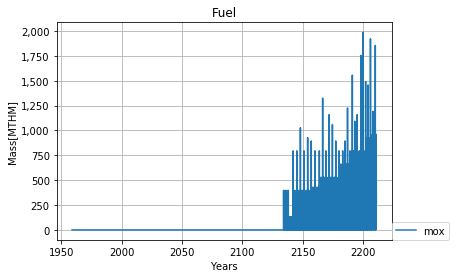
\includegraphics[scale=0.6]{./images/mox_fuel.png}
	\end{center}
	\caption{\gls{MOX} fuel demand for EG29}
	\label{fig:mox}
\end{figure}
\begin{figure}[htbp!]
	\begin{center}
		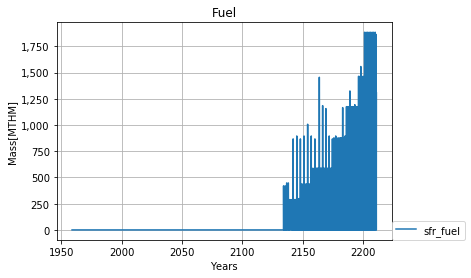
\includegraphics[scale=0.6]{./images/sfr_fuel.png}
	\end{center}
	\caption{\gls{SFR} fuel demand for EG29}
	\label{fig:sfr}
\end{figure}
\FloatBarrier

\Cref{fig:mox} and \cref{fig:sfr} plot the fuel demand of \gls{MOX} \glspl{LWR} and \glspl{SFR},
respectively, in an EG29 scenario.





\subsection{Static Parameters}
Various parameters, most notably throughput and capacity values of fuel cycle support facilities,
need to adjust according to demand. With transition scenarios with increasing power demand, the 
demand for fuel and fissile material generally increases over time. The current workaround is to either
have a facility with infinite capacity, or to set the capacity to a manually-calculated (look-back method)
maximum fuel demand. The infinite capacity method fails for EG29 and EG30, due to the greedy exchange
model. The look-back method allows a complete simulation, but inefficiencies occur with the distribution
of fissile material, since the facility with the higher demand has to fill up first in order for the facility
with the lower demand to receive fissile material. 

A fix for this is to have a dynamic throughput that adjusts according
to predicted fuel demand, or, more realistically, have an archetype with fixed, reasonable, throughput/buffer
that is deployed when there is fuel demand beyond its predicted throughput.

\subsection{Individual Demand Estimation}
Currently, the \Cyclus framework's market is completely agent-based. At every timestep, each agent `submits' its
demand and supply and the trade is made. However, this individual frame can cause inefficiencies mentioned previously.
A more efficient process would be to set all demands proportional to the fuel demand. An example is illustrated
in \cref{diag:hd}.

% Define block styles
\tikzstyle{decision} = [diamond, draw, fill=blue!20, 
text width=4.5em, text badly centered, node distance=3cm, inner sep=0pt]
\tikzstyle{block} = [rectangle, draw, fill=blue!20, 
text width=5em, text centered, rounded corners, minimum height=4em]
\tikzstyle{line} = [draw, -latex']
\tikzstyle{cloud} = [draw, ellipse,fill=red!20, node distance=3cm,
minimum height=2em]


\begin{figure}
	\centering
	\scalebox{0.7}{
		\begin{tikzpicture}[align=center, node distance = 3cm and 3cm, auto]
		% Place nodes
		\node [block] (rea) {\texttt{Reactor}};
		\node [cloud, below of=rea] (d1) {1. Demand: \textbf{Fuel}};
		\node [cloud, below of=d1] (s1) {2. Change throughput to \textbf{Fuel}};
		\node [block, below of=s1] (ff) {\texttt{FuelFab}};
		\node [cloud, below of=ff] (d2) {3. Demand: Fissile Material ($\propto \textbf{Fuel}$)};		
		\node [cloud, below of=d2] (s2) {4. Change capacity to ($\propto \textbf{Fuel}$)};
		\node [block, below of=s2] (rep) {\texttt{Separations}};
		
		
		\draw[->, thick] (rea) -- (d1);
		\draw[->, thick] (d1) -- (s1);
		\draw[->, thick] (s1) -- (ff);
		\draw[->, thick] (ff) -- (d2);
		\draw[->, thick] (d2) -- (s2);
		\draw[->, thick] (s2) -- (rep);
		\end{tikzpicture}
		
	}
	\caption{Fuel-centered Demand Logic Flow}
	\label{diag:hd}
\end{figure}
 

\subsection{A Need For Market-Peeking}
The \Cyclus framework can benefit greatly from a market-peeking capability,
where each agent can query the market (previous transactions or demand) to adjust its parameters. For example, fuel fabrication
agents can query the previous (or, eventually, expected) demand of fuel and adjust their throughputs to meet the demand. 
The market-peeking capability is essential for demand-prediction models.

Moreover, with the market-peeking capability, support facilities can estimate adjust their
capacities by estimating
the demand of fuel/fissile material proportional to power demand (`power' is a market commodity in \Cyclus).

\subsection{A Need For Inter-Agent Feedback}
Inter-agent feedback means that agents can communicate with each other and change its parameters accordingly. 
For example, an increase in fabrication capacity, should cause an increase in reprocessing capacity. Also,
if a reactor is shutdown due to lack of fuel, this should cause a flag to increase fabrication capacity,
or `investigate'
This would be problematic in parallel to the market-peeking capability, since there would be more than one algorithm
that changes the throughput of an agent. 

\subsection{Irresponsible deployment}
The \textsc{DeployInst}\xspace model deploys prototypes in a user-defined time period, even though there is not 
enough fuel to operate the reactor. The deployed reactor is remains idle if the fuel supply is short. Deploying new reactors
without sufficient fissile material to support it can cause other already-deployed reactors without fuel, causing
a cascade of shutdowns. Using the market-peeking or feedback capability, new reactors should be deployed only
if there is sufficient fuel to support the startup of the reactor as well as currently deployed reactors. 


\section{Additional Possible Improvements}
Though not critical to the current goal, having the following capabilities can increase
the accuracy of simulations.


\subsection{Blanket capability for \textsc{Reactor}\xspace}
For \glspl{SFR}, the blanket and the driver have different effective fuel residence times, meaning that
they should (ideally) be discharged and loaded separately. However, with current capabilities, the option is the average
the mass and composition of driver and blanket to treat is as one commodity.

\subsection{Depletion Calculations}
Depletion calculations are done outside of the simulation. However, if advanced reactor models like \textsc{Cyborg}\xspace
or \textsc{Bright-Lite}\xspace are utilized, there could be more accurate depletion calculations and 
perhaps dynamic Breeding Ratio modeling.

\subsection{\textsc{Reactor}\xspace Decommissioning Behavior}
The \Cycamore \textsc{Reactor}\xspace, when decommissioned mid-cycle, transmutes half of
its current assemblies, and discharges all its core as waste commodity. This is in order to model the average
composition of discharged assemblies in different stages. An alternative would
be to have recipes for each stage (ie. for four batch, there would be three spent fuel recipes).


\bibliographystyle{abbrv}
\bibliography{bibliography}


\end{document}